\input /Users/davidmcallester/ICloude/tex/SlidePreamble
\input /Users/davidmcallester/ICloude/tex/preamble


\begin{document}

{\Huge

  \centerline{\bf TTIC 31230, Fundamentals of Deep Learning}
  \bigskip
  \centerline{David McAllester, Autumn 2021}
  \vfill
  \vfil
  \centerline{Vector Quantized Variational Autoencoders (VQ-VAEs)}
  \vfill
  \vfill
\slide{Gaussian VAEs}

\vfill
\begin{eqnarray*}
\mbox{VAE:}\;\;\;\Phi^*,\Psi^* &  = & \argmin_{\Phi,\Psi}\;E_{y,z}  \;\ln \frac{\hat{p}_\Psi(z|y)}{p_\Phi(z)}  - \ln p_\Phi(y|z) \\
\end{eqnarray*}

\vfill
All models are Gaussian densities.

\vfill
{\huge 
\begin{eqnarray*}
p_\Phi(z[i]) & \propto & \exp((z[i]-\mu_\Phi[i])^2/2\sigma^2_\Phi[i])\\
\\
p_\Psi(z[i]|y) & \propto & \exp((z[i]-\hat{z}_\Psi(y)[i])^2/2\sigma^2_\Psi(y)[i])\\
\\
p_\Phi(y[i]|z) & \propto & \exp((y[i]-\hat{y}_\Phi(z)[i])^2/2\sigma_\Phi^2(z)[i])\\
\end{eqnarray*}
}

\slide{WLOG $p_\Phi(z) = {\cal N}(0,I)$}


There is a simple reparameterization $\Phi'$ and $\Psi'$ of $\Phi$ and $\Psi$ such that $\Phi'$ and $\Psi'$ give the same value of the ELBO
but $p_{\Phi'}(z) = {\cal N}(0,I)$.

\ignore{
\vfill
{\huge
\begin{eqnarray*}
KL_\Phi & = & \sum_i \;\frac{ \sigma_\Phi(y)[i]^2 +(\mu_\Phi(y)[i] - \mu_z[i])^2}{2\sigma_z[i]^2}
+ \ln\frac{\sigma_z[i]}{\sigma_\Phi(y)[i]} - \frac{1}{2}
\\
KL_{\Phi'} & = & \sum_i \;\frac{\sigma_{\Phi'}(y)[i]^2 +\mu_{\Phi'}(y)[i]^2}{2} + \ln\frac{1}{\sigma_{\Phi'}(y)[i]} - \frac{1}{2}
\end{eqnarray*}

Setting $\Phi'$ so that
\begin{eqnarray*}
\mu_{\Phi'}(y)[i] & = & (\mu_\Phi(y)[i] - \mu_z[i])/\sigma_z[i] \\
\sigma_{\Phi'}(y)[i] & = & \sigma_\Phi(y)[i]/\sigma_z[i]
\end{eqnarray*}

\vfill
gives {\color{red} $KL(\hat{p}_{\Phi}(z|y),p_\Phi(z)) = KL(\hat{p}_{\Phi'}(z|y),{\cal N}(0,I))$}.
}
}
\slide{Gaussian VAEs for Faces 2014}

We can sample faces from the VAE by sampling noise $z$ from $p_\Phi(z)$ and then sampling an image $y$ from $p_\Phi(y|z)$.

\vfill
\centerline{\includegraphics[width = 3in]{\images/VariationalFaces}}
\centerline{[Alec Radford]}

\slide{VQ-VAEs 2019}

\centerline{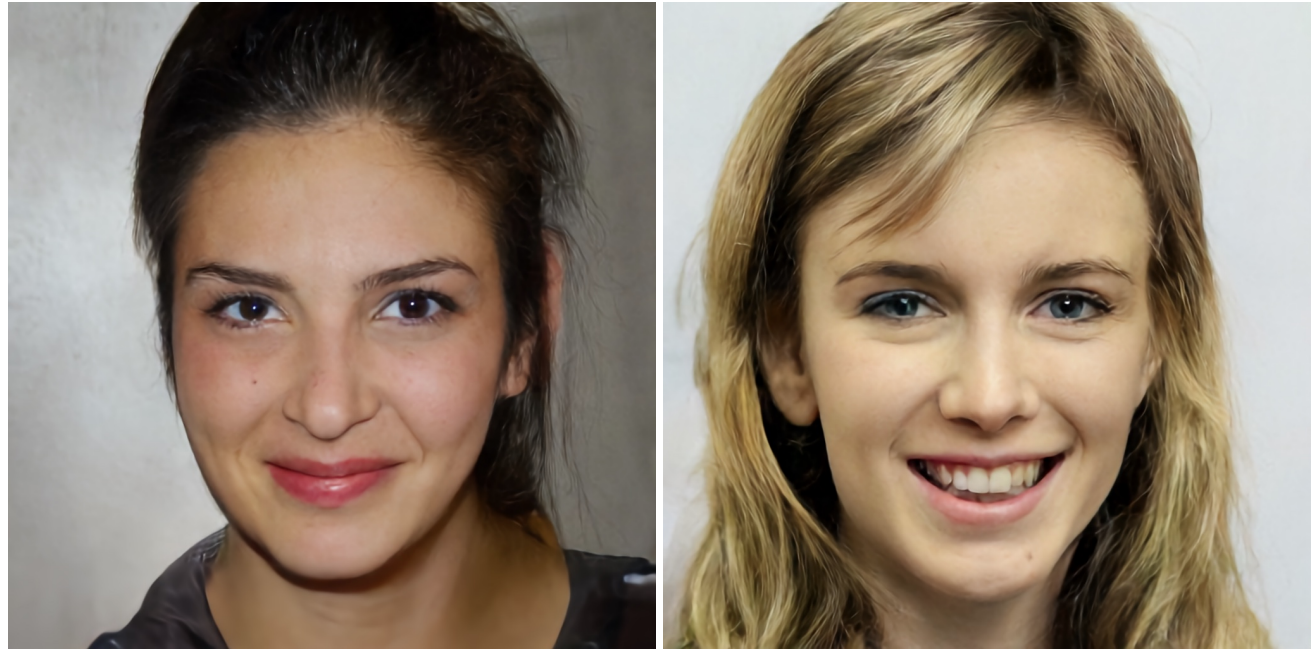
\includegraphics[width = 8in]{\images/VQ-VAE22}}

\vfill
VQ-VAE-2, Razavi et al. June, 2019

\slide{VQ-VAEs 2019}

\centerline{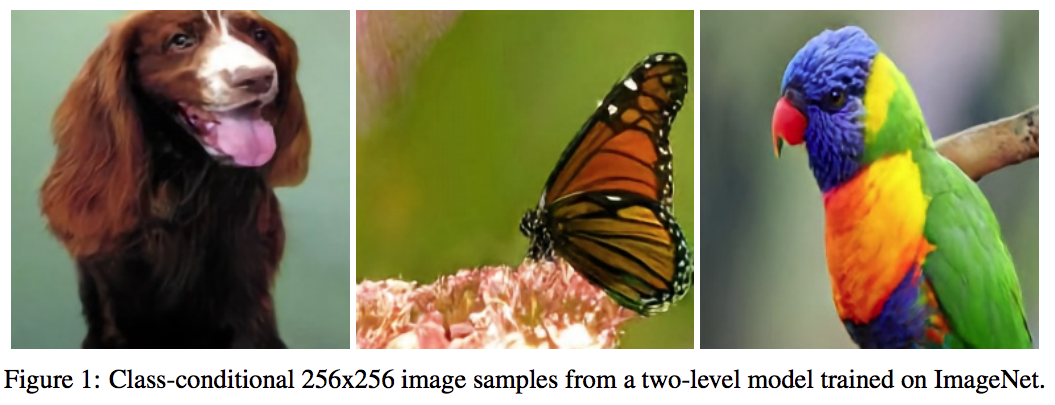
\includegraphics[width = 10in]{\images/VQ-VAE21}}

\vfill
VQ-VAE-2, Razavi et al. June, 2019

\slide{Vector Quantized VAEs (VQ-VAE)}

VQ-VAEs effectively perform $k$-means on vectors in the model so as to represent vectors by discrete cluster centers.

\vfill
We use $x$ and $y$ for spatial image coordinates and use $s$ (for signal) to denote images.

\slide{VQ-VAE Encoder-Decoder}

\centerline{\includegraphics[width =5in]{\images/VQCodes}}

\vfill
In the one-layer case the latent variable (compressed image) is a ``symbolic image'' $z[X,Y]$ where $z[x,y]$ is a symbol (a cluster index).

\vfill
Naively $z[X,Y]$ can be represented with $XY \log_2 K$ bits.

\slide{VQ-VAE Image Sampler}

\centerline{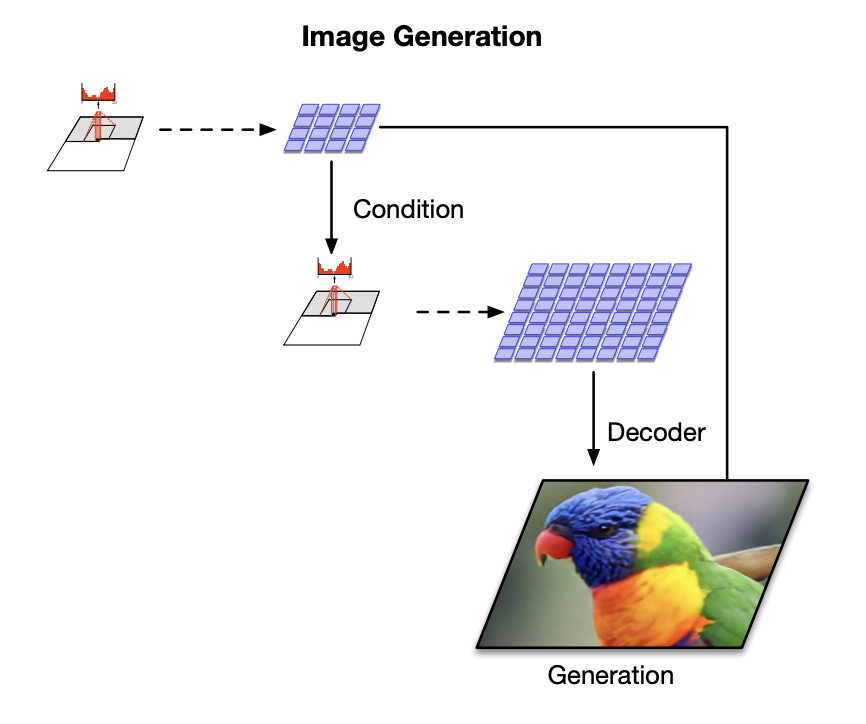
\includegraphics[height =2in]{\images/VQSampler}}

But they also train an autoregressive probability model (pixel CNN) giving a probability $P_\Phi(z[X,Y])$ for the symbolic image $z[X,Y]$.

\vfill
This gives  $-\log_2 P_\Phi(z[X,Y])$ bits per image (much lower).

\vfill
To sample an image they sample $z[X,Y]$ from $P_\Phi(z[X,Y])$.


\slide{VQ-VAE Encode-Decode Training}

We train a code book $C[K,I]$ where $C[k,I]$ is the center vector of cluster $k$.

{\huge
\begin{eqnarray*}
L[X,Y,I] & = & \mathrm{Enc}_\Phi(s) \\
\\
z[x,y] & = & \argmin_k \;||L[x,y,I] - C[k,I]|| \\
\\
\hat{L}[x,y,I] & = & C[z[x,y],I] \\
\\
\hat{s} & = & \mathrm{Dec}_\Phi(\hat{L}[X,Y,I])
\end{eqnarray*}
}

\vfill
The ``symbolic image'' $z[X,Y]$ is the latent variable (compressed image) with naive bit length $XY\log_2 K$.

\slide{Training the Code Book}

We preserve information about the image $s$ by minimizing the distortion between $L[X,Y,I]$ and its reconstruction $\hat{L}[X,Y,I]$.

\vfill
\begin{eqnarray*}
\Phi^* & = & \argmin_\Phi \;E_s\; \beta||L[X,Y,I] - \hat{L}[X,Y,I]||^2 + ||s -\hat{s}||^2
\end{eqnarray*}

\slide{Parameter-Specific Learning Rates}

$$||L[X,Y,I] - \hat{L}[X,Y,I]||^2 = \sum_{x,y}\;||L[x,y,I] - C[z[x,y],I]||^2$$

\vfill
For the gradient of this they use

\begin{eqnarray*}
\mathrm{for}\;x,y\;\;L[x,y,I].\grad & \pluseq & 2\beta({L}[x,y,I]- C[z[x,y],I]) \\
\mathrm{for}\;x,y\;\;C[z[x,y],I].\grad & \pluseq & 2(C[z[x,y],I] - L[x,y,I])
\end{eqnarray*}

\vfill
This gives a parameter-specific learning rate for $C[K,I]$.

\vfill
Parameter-specific learning rates do not change the stationary points (the points where the gradients are zero).

\slide{The Relationship to $K$-means}

\begin{eqnarray*}
\mathrm{for}\;x,y\;\;C[z[x,y],I].\grad & \pluseq & 2(C[z[x,y],I] - L[x,y,I])
\end{eqnarray*}

\vfill
At a stationary point we get that $C[k,I]$ is the mean of the set of vectors $L[x,y,I]$ with $z[x,y] = k$ (as in $K$-means).

\slide{Straight Through Gradients}


{\huge
\begin{eqnarray*}
z[x,y] & = & \argmin_k \;||L[x,y,I] - C[k,I]|| \\
\\
\hat{L}[x,y,I] & = & C[z[x,y],I]
\end{eqnarray*}
}
$z[x,y].\grad = 0$ and back-propagation fails.  This is true for any discrete value in a network.

\vfill
They use ``straight-through'' gradients.

\begin{eqnarray*}
\mathrm{for}\;x,y\;\;L[x,y,I].\grad & \pluseq & \hat{L}[x,y,I].\grad
\end{eqnarray*}

\vfill
This assumes low distortion between $L[X,Y,I]$ and $\hat{L}[X,Y,I]$.

\slide{A Suggested Modification}

The parameter $\beta$ is paying two roles

\vfill
\begin{itemize}
\item It controls the relative weight of the two distortion losses.

\vfill
\item It controls the learning rate adjustment for the codebook.
\end{itemize}

\vfill
Shouldn't we have separate parameters for these two roles?

\slide{Multi-Layer Vector Quantized VAEs}
\centerline{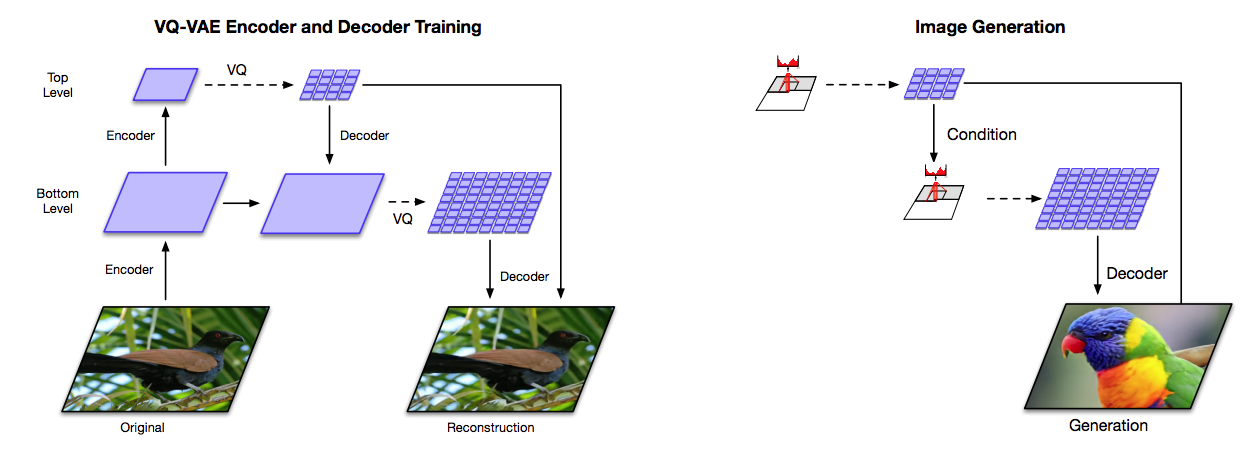
\includegraphics[width =10in]{\images/VQ-VAE24}}

\slide{Quantitative Evaluation}

The VQ-VAE2 paper reports a classification accuracy score (CAS) for class-conditional image generation.

\vfill
We generate image-class pairs from the generative model trained on the ImageNet training data.

\vfill
We then train an image classifier from the generated pairs and measure its accuracy on the ImageNet test set.

\vfill
\centerline{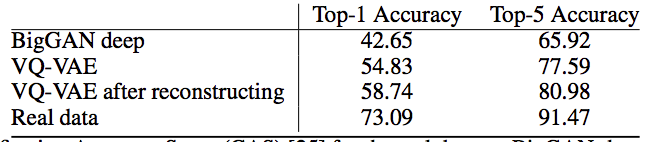
\includegraphics[width=7in]{\images/VQ-VAE23}}

\slide{Image Compression}

\vfill
\centerline{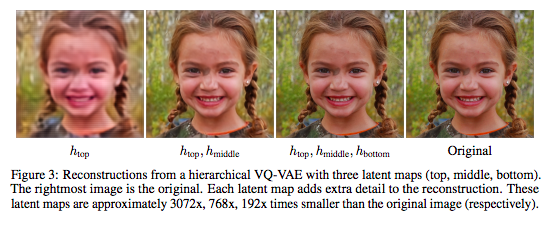
\includegraphics[width = 10in]{\images/VQgirl}}

\slide{Rate-Distortion Evaluation.}

Rate-distortion metrics for image compression to discrete representations support unambiguous rate-distortion evaluation.

\vfill
Rate-distortion metrics also allow one to explore the rate-distortion trade-off.

\vfill
\centerline{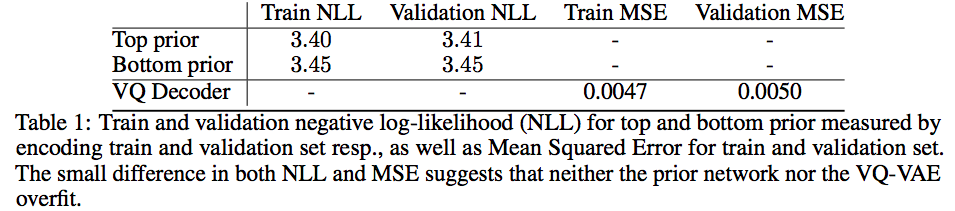
\includegraphics[width = 10in]{\images/VQVAE2Scores}}

\slide{DALL$\cdot$E: A Text-Conditional Image dVAE}
\vfill
DALL$\cdot$E is a text-conditional VQ-VAE model of images.

\vfill
The Vector quantization is done independent of the text.  However, the model of the probability distribution of the symbolic image $z[x,y]$ is conditioned on text.

\vfill
\centerline{\huge Ramesh et al. 2021}

\slide{DALL$\cdot$E}

\centerline{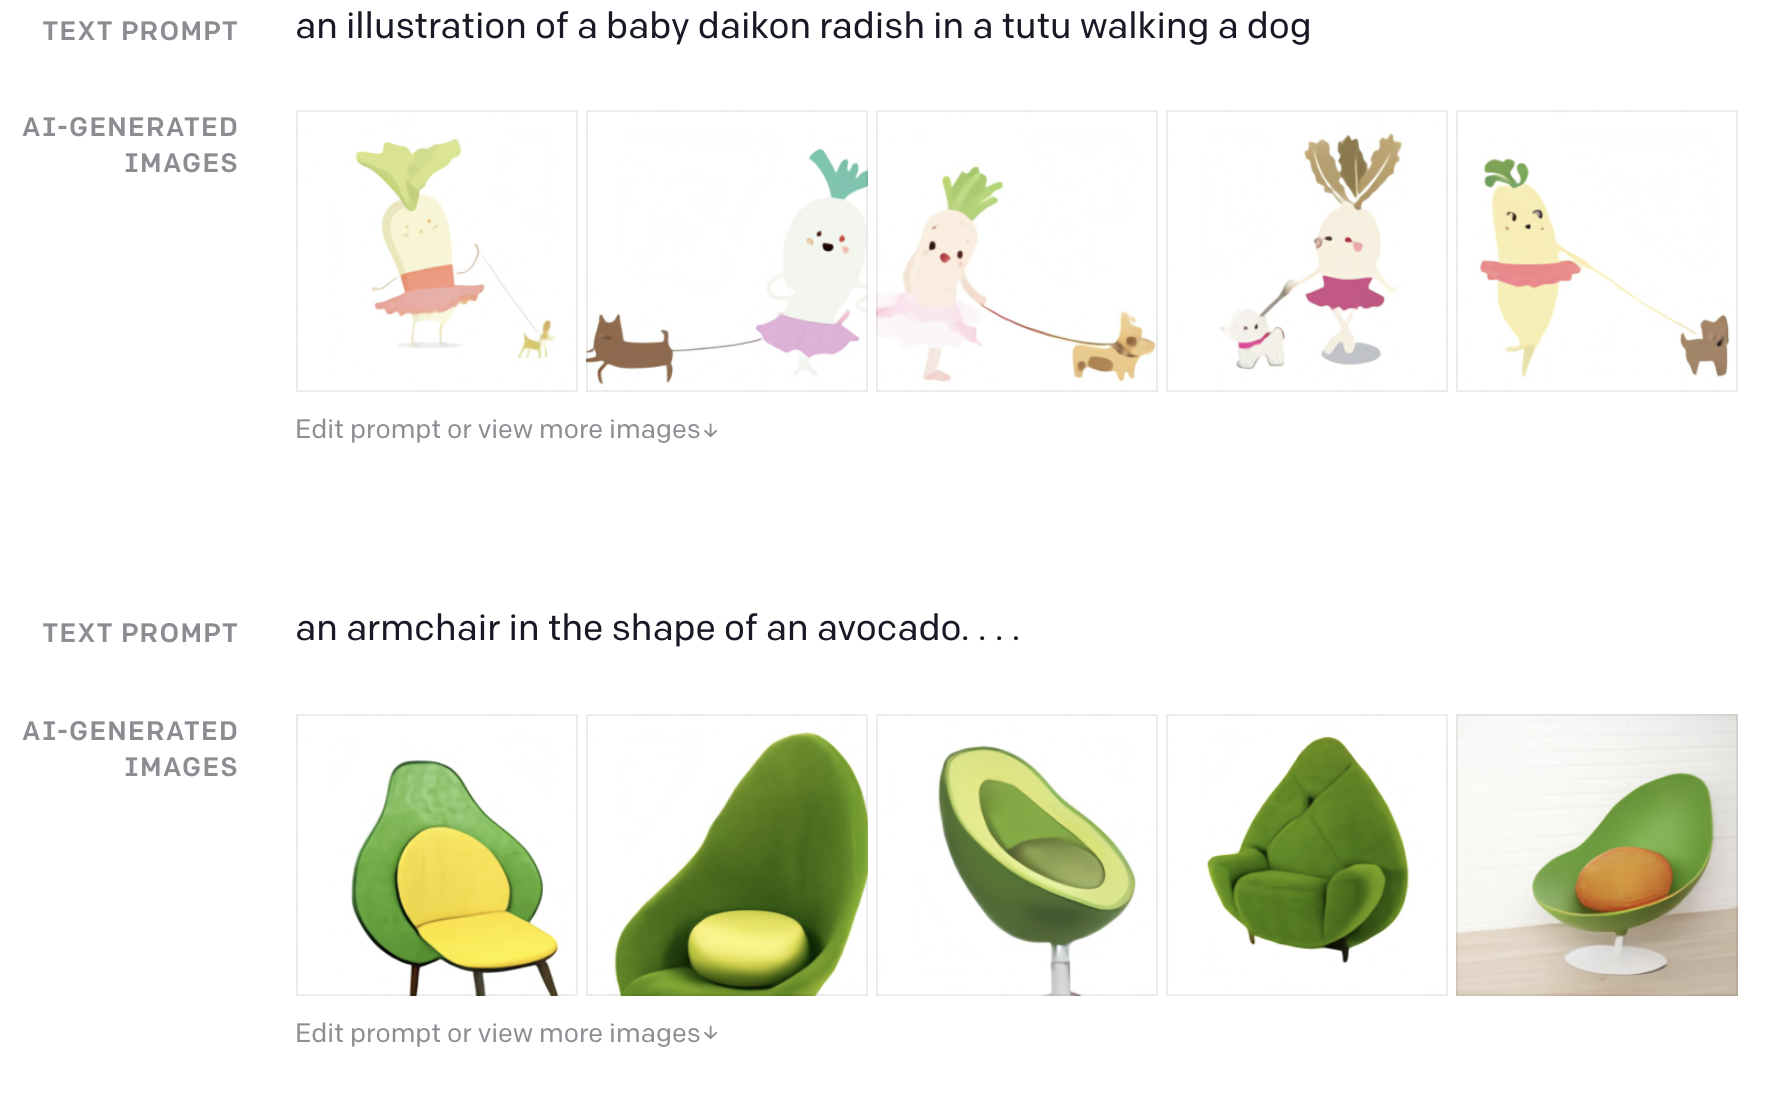
\includegraphics[height= 5.5in]{\images/DALLE1}}

\slideplain{END}

\end{document}
